\section*{Problem Statement}
The objective of this problem is to approximate the value of $\sin(35^\circ)$
using Newton–Gregory forward interpolation. The interpolation is based on support
points of the sine function sampled every $10^\circ$ between $0^\circ$ and $180^\circ$.

\begin{quote}
  \textbf{NOTE}: The code can be accessed using this link: \href{https://raw.githubusercontent.com/HavokSahil/computational-techniques-assignments/refs/heads/main/assignment4/a3.m}{MATLAB}, \href{https://raw.githubusercontent.com/HavokSahil/computational-techniques-assignments/refs/heads/main/assignment4/a3.jl}{Julia}.
\end{quote}


\section*{Methodology}
Newton–Gregory forward interpolation constructs a polynomial approximation for
functions sampled at equally spaced points. Let the support points be
\[
x_0, x_1, \dots, x_{N-1}, \quad y_i = f(x_i),
\]
with spacing $h = x_{i+1} - x_i$. The forward difference table is defined as:
\[
\Delta y_i = y_{i+1} - y_i, \quad
\Delta^2 y_i = \Delta y_{i+1} - \Delta y_i, \quad \dots
\]

The interpolation polynomial is given by:
\[
P(x) = y_0 + \frac{u}{1!}\Delta y_0 + \frac{u(u-1)}{2!}\Delta^2 y_0
       + \cdots + \frac{u(u-1)\cdots(u-k+1)}{k!}\Delta^k y_0,
\]
where
\[
u = \frac{x - x_0}{h}.
\]

\subsection*{Pseudo-code}
\begin{enumerate}
  \item Define spacing $h = \pi/18$ (corresponding to $10^\circ$).
  \item Construct support points $\theta_i = 0:h:\pi$, $y_i = \sin(\theta_i)$.
  \item Build the forward-difference table for $y_i$.
  \item For an arbitrary $x$:
  \begin{enumerate}
    \item Compute $u = (x-x_0)/h$.
    \item Evaluate the polynomial using the Newton–Gregory formula.
  \end{enumerate}
  \item Plot the interpolated polynomial and highlight $\sin(35^\circ)$.
\end{enumerate}

\section*{Results}
The sine function was interpolated from support points spaced $10^\circ$ apart.
The following were observed:
\begin{itemize}
  \item Black markers: true $\sin(x)$ at multiples of $10^\circ$.
  \item Black curve: interpolated polynomial passing through all support points.
  \item Red marker: interpolated estimate of $\sin(35^\circ)$.
\end{itemize}

The computed interpolated value is:
\[
\sin(35^\circ) \approx 0.564642,
\]
while the exact value is
\[
\sin(35^\circ) \approx 0.573576.
\]

\begin{figure}[h!]
  \centering
  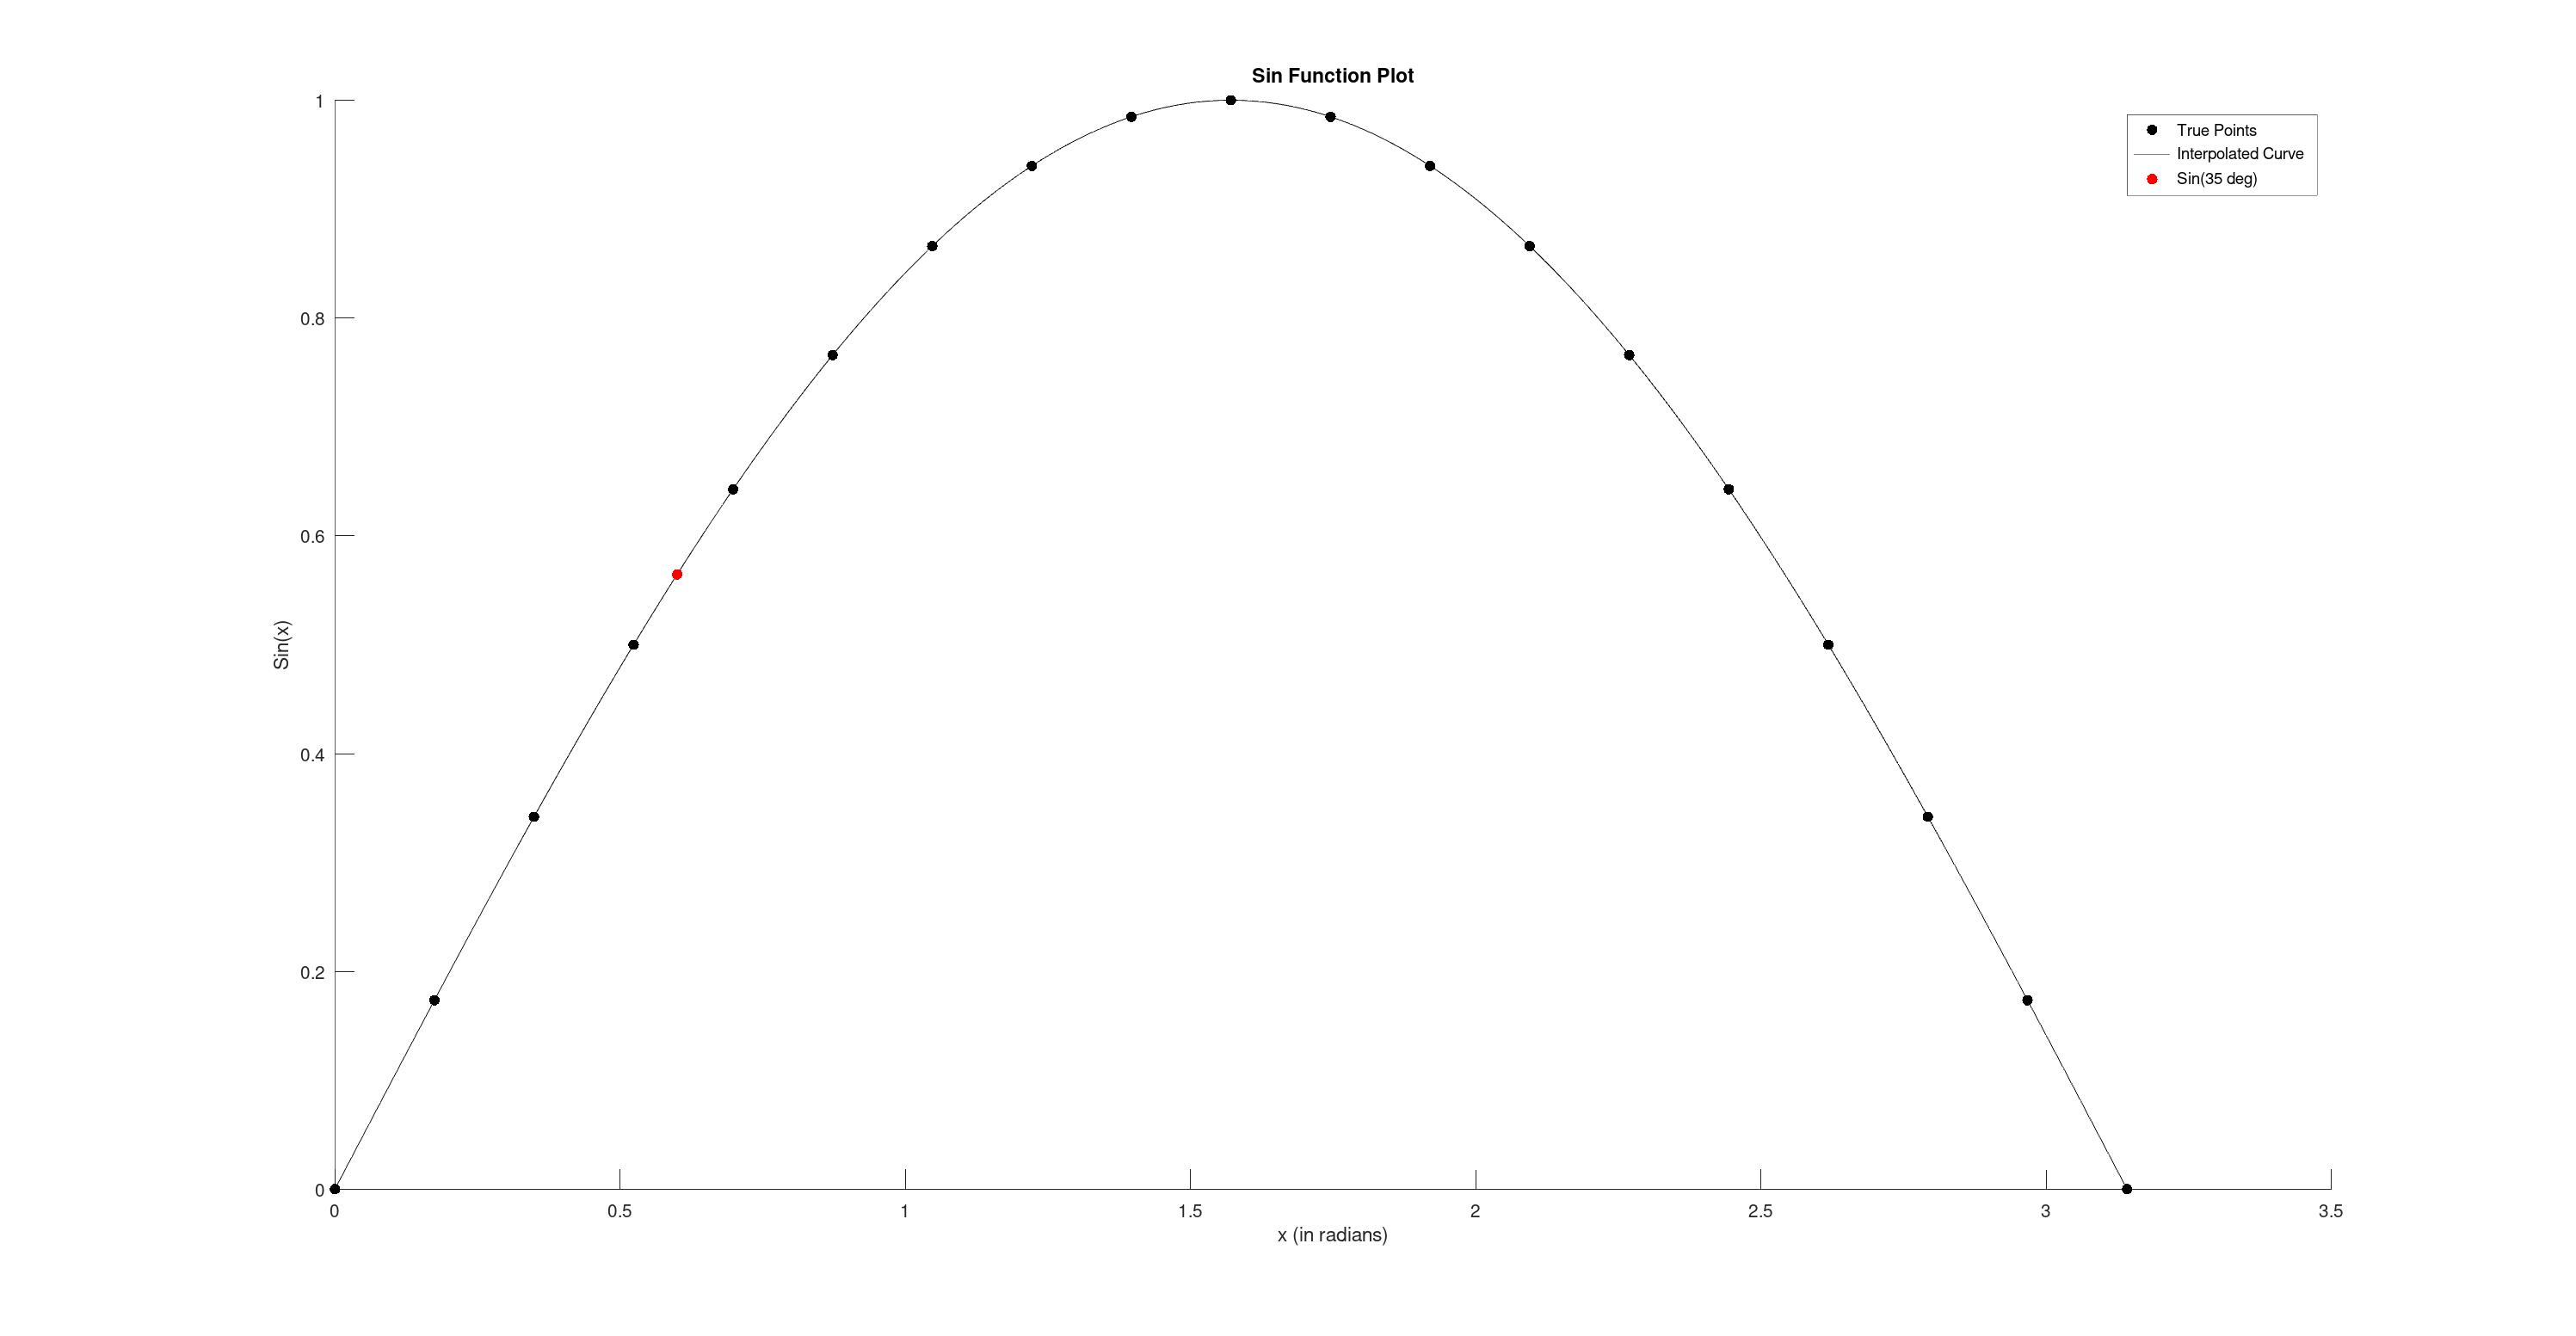
\includegraphics[width=0.75\textwidth]{a3.jpg}
  \caption{Newton–Gregory interpolation of $\sin(x)$ using $10^\circ$ spaced support data.}
\end{figure}

\section*{Conclusion}
Newton–Gregory forward interpolation approximately reconstructed the sine function
from $10^\circ$ spaced support data. The interpolated estimate at $35^\circ$
is fairly close to the exact sine value, validating the method’s effectiveness for
smooth functions.
